% Figure 2: Ablation bar chart — 8 conditions × 3 puzzles
%
% DEPENDENCIES: main.tex must include:
%   \usepackage{tikz}
%   \usepackage{pgfplots}
%   \usepgflibrary{patterns}
%   \pgfplotsset{compat=1.18}
%
% Colors by condition type:
%   C0  light gray    (bare baseline)
%   C1  medium gray   (rubric only)
%   C2  light blue    (principles compact)
%   C3  medium blue   (principles full)
%   C4  green         (philosophy only)
%   C5  orange        (lens only)
%   C6  dark blue     (full profile — current system)
%   C7  dark gray     (profile + principles)

\begin{figure}[t]
\centering
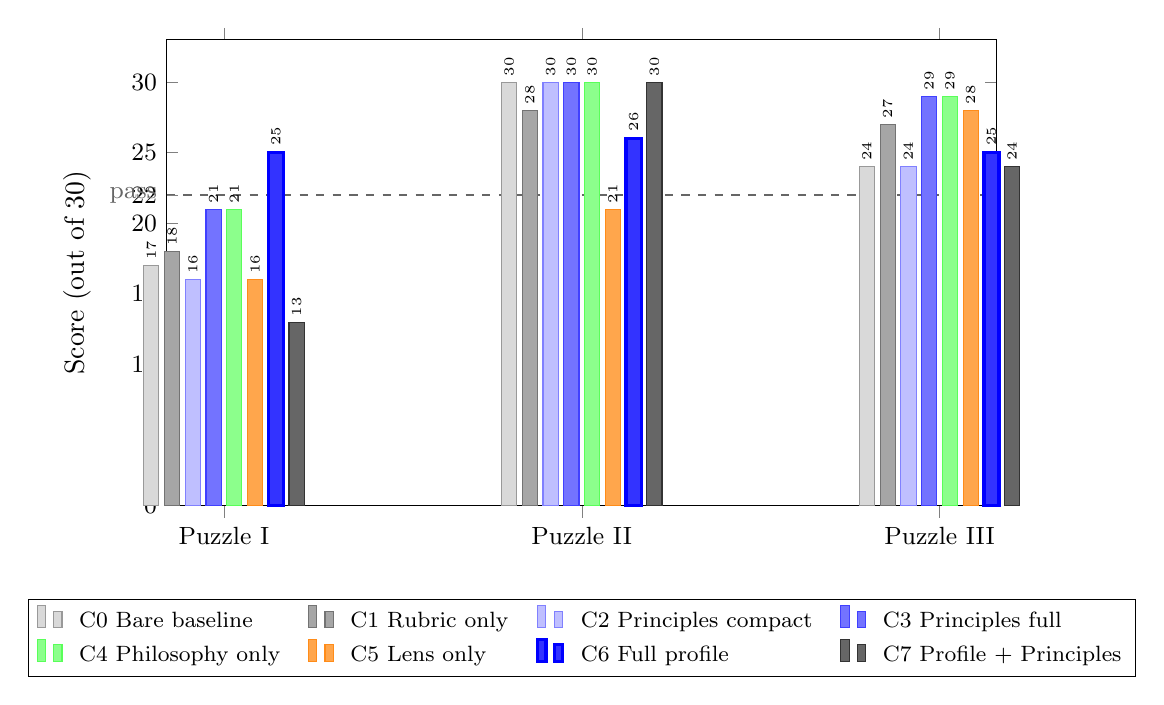
\begin{tikzpicture}
\begin{axis}[
    ybar,
    bar width=5.5pt,
    width=\textwidth,
    height=7.5cm,
    enlarge x limits=0.08,
    ylabel={Score (out of 30)},
    ymin=0,
    ymax=33,
    ytick={0,5,10,15,20,22,25,30},
    yticklabel style={font=\small},
    extra y ticks={22},
    extra y tick style={
        grid=major,
        grid style={dashed, thick, black!60},
        tick label style={font=\small\itshape, color=black!60}
    },
    extra y tick labels={pass},
    symbolic x coords={Puzzle I, Puzzle II, Puzzle III},
    xtick=data,
    xticklabel style={font=\small},
    legend style={
        at={(0.5,-0.20)},
        anchor=north,
        legend columns=4,
        font=\footnotesize,
        column sep=4pt,
        /tikz/every even column/.append style={column sep=8pt},
    },
    legend cell align=left,
    nodes near coords,
    nodes near coords style={font=\tiny, rotate=90, anchor=west, inner sep=2pt},
    nodes near coords align={vertical},
    every node near coord/.append style={/pgf/number format/.cd, fixed, precision=0},
    grid=none,
    axis on top=false,
    clip=false,
]

% C0 — Bare baseline — light gray
\addplot[fill=black!15, draw=black!40] coordinates {
    (Puzzle I,  17)
    (Puzzle II, 30)
    (Puzzle III,24)
};

% C1 — Rubric only — medium gray
\addplot[fill=black!35, draw=black!55] coordinates {
    (Puzzle I,  18)
    (Puzzle II, 28)
    (Puzzle III,27)
};

% C2 — Principles compact — light blue
\addplot[fill=blue!25, draw=blue!50] coordinates {
    (Puzzle I,  16)
    (Puzzle II, 30)
    (Puzzle III,24)
};

% C3 — Principles full — medium blue
\addplot[fill=blue!55, draw=blue!75] coordinates {
    (Puzzle I,  21)
    (Puzzle II, 30)
    (Puzzle III,29)
};

% C4 — Philosophy only — green
\addplot[fill=green!45, draw=green!65] coordinates {
    (Puzzle I,  21)
    (Puzzle II, 30)
    (Puzzle III,29)
};

% C5 — Lens only — orange
\addplot[fill=orange!70, draw=orange!90] coordinates {
    (Puzzle I,  16)
    (Puzzle II, 21)
    (Puzzle III,28)
};

% C6 — Full profile (current system) — dark blue, prominent
\addplot[fill=blue!80, draw=blue!100, line width=1.2pt] coordinates {
    (Puzzle I,  25)
    (Puzzle II, 26)
    (Puzzle III,25)
};

% C7 — Profile + Principles — dark gray
\addplot[fill=black!60, draw=black!80] coordinates {
    (Puzzle I,  13)
    (Puzzle II, 30)
    (Puzzle III,24)
};

\legend{
    C0 Bare baseline,
    C1 Rubric only,
    C2 Principles compact,
    C3 Principles full,
    C4 Philosophy only,
    C5 Lens only,
    C6 Full profile,
    C7 Profile + Principles
}

\end{axis}
\end{tikzpicture}

% Annotation strip below the chart
\vspace{4pt}
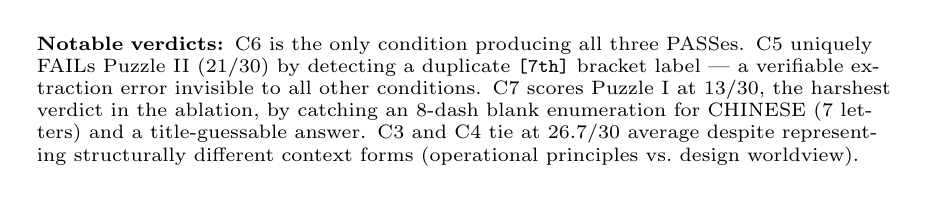
\begin{tikzpicture}[font=\scriptsize]
\node[anchor=west, text width=0.9\textwidth, align=left] at (0,0) {%
    \textbf{Notable verdicts:}
    C6 is the only condition producing all three PASSes.
    C5 uniquely FAILs Puzzle~II (21/30) by detecting a duplicate \texttt{[7th]} bracket label --- a verifiable extraction error invisible to all other conditions.
    C7 scores Puzzle~I at 13/30, the harshest verdict in the ablation, by catching an 8-dash blank enumeration for CHINESE (7 letters) and a title-guessable answer.
    C3 and C4 tie at 26.7/30 average despite representing structurally different context forms (operational principles vs.\ design worldview).%
};
\end{tikzpicture}

\caption{Score by condition and puzzle across the 8-condition ablation. All conditions produce 0 named frameworks in C0--C1; C2 introduces principle-name vocabulary; C3--C7 produce domain-specific analytical frameworks. The pass threshold (22/30, dashed) shows that only C6 (full profile) produces consistent passes across all three puzzles. C5 uniquely detects a verifiable defect in Puzzle~II; C7 scores Puzzle~I harshest by catching a factual error.}
\label{fig:ablation}
\end{figure}
